\section{Tutorial}

\begin{frame}
  \tableofcontents[currentsection] 
\end{frame}


\begin{frame}[fragile]

\centerline{\bf Example -- Pendulum}

\begin{minipage}{0.35\textwidth}
    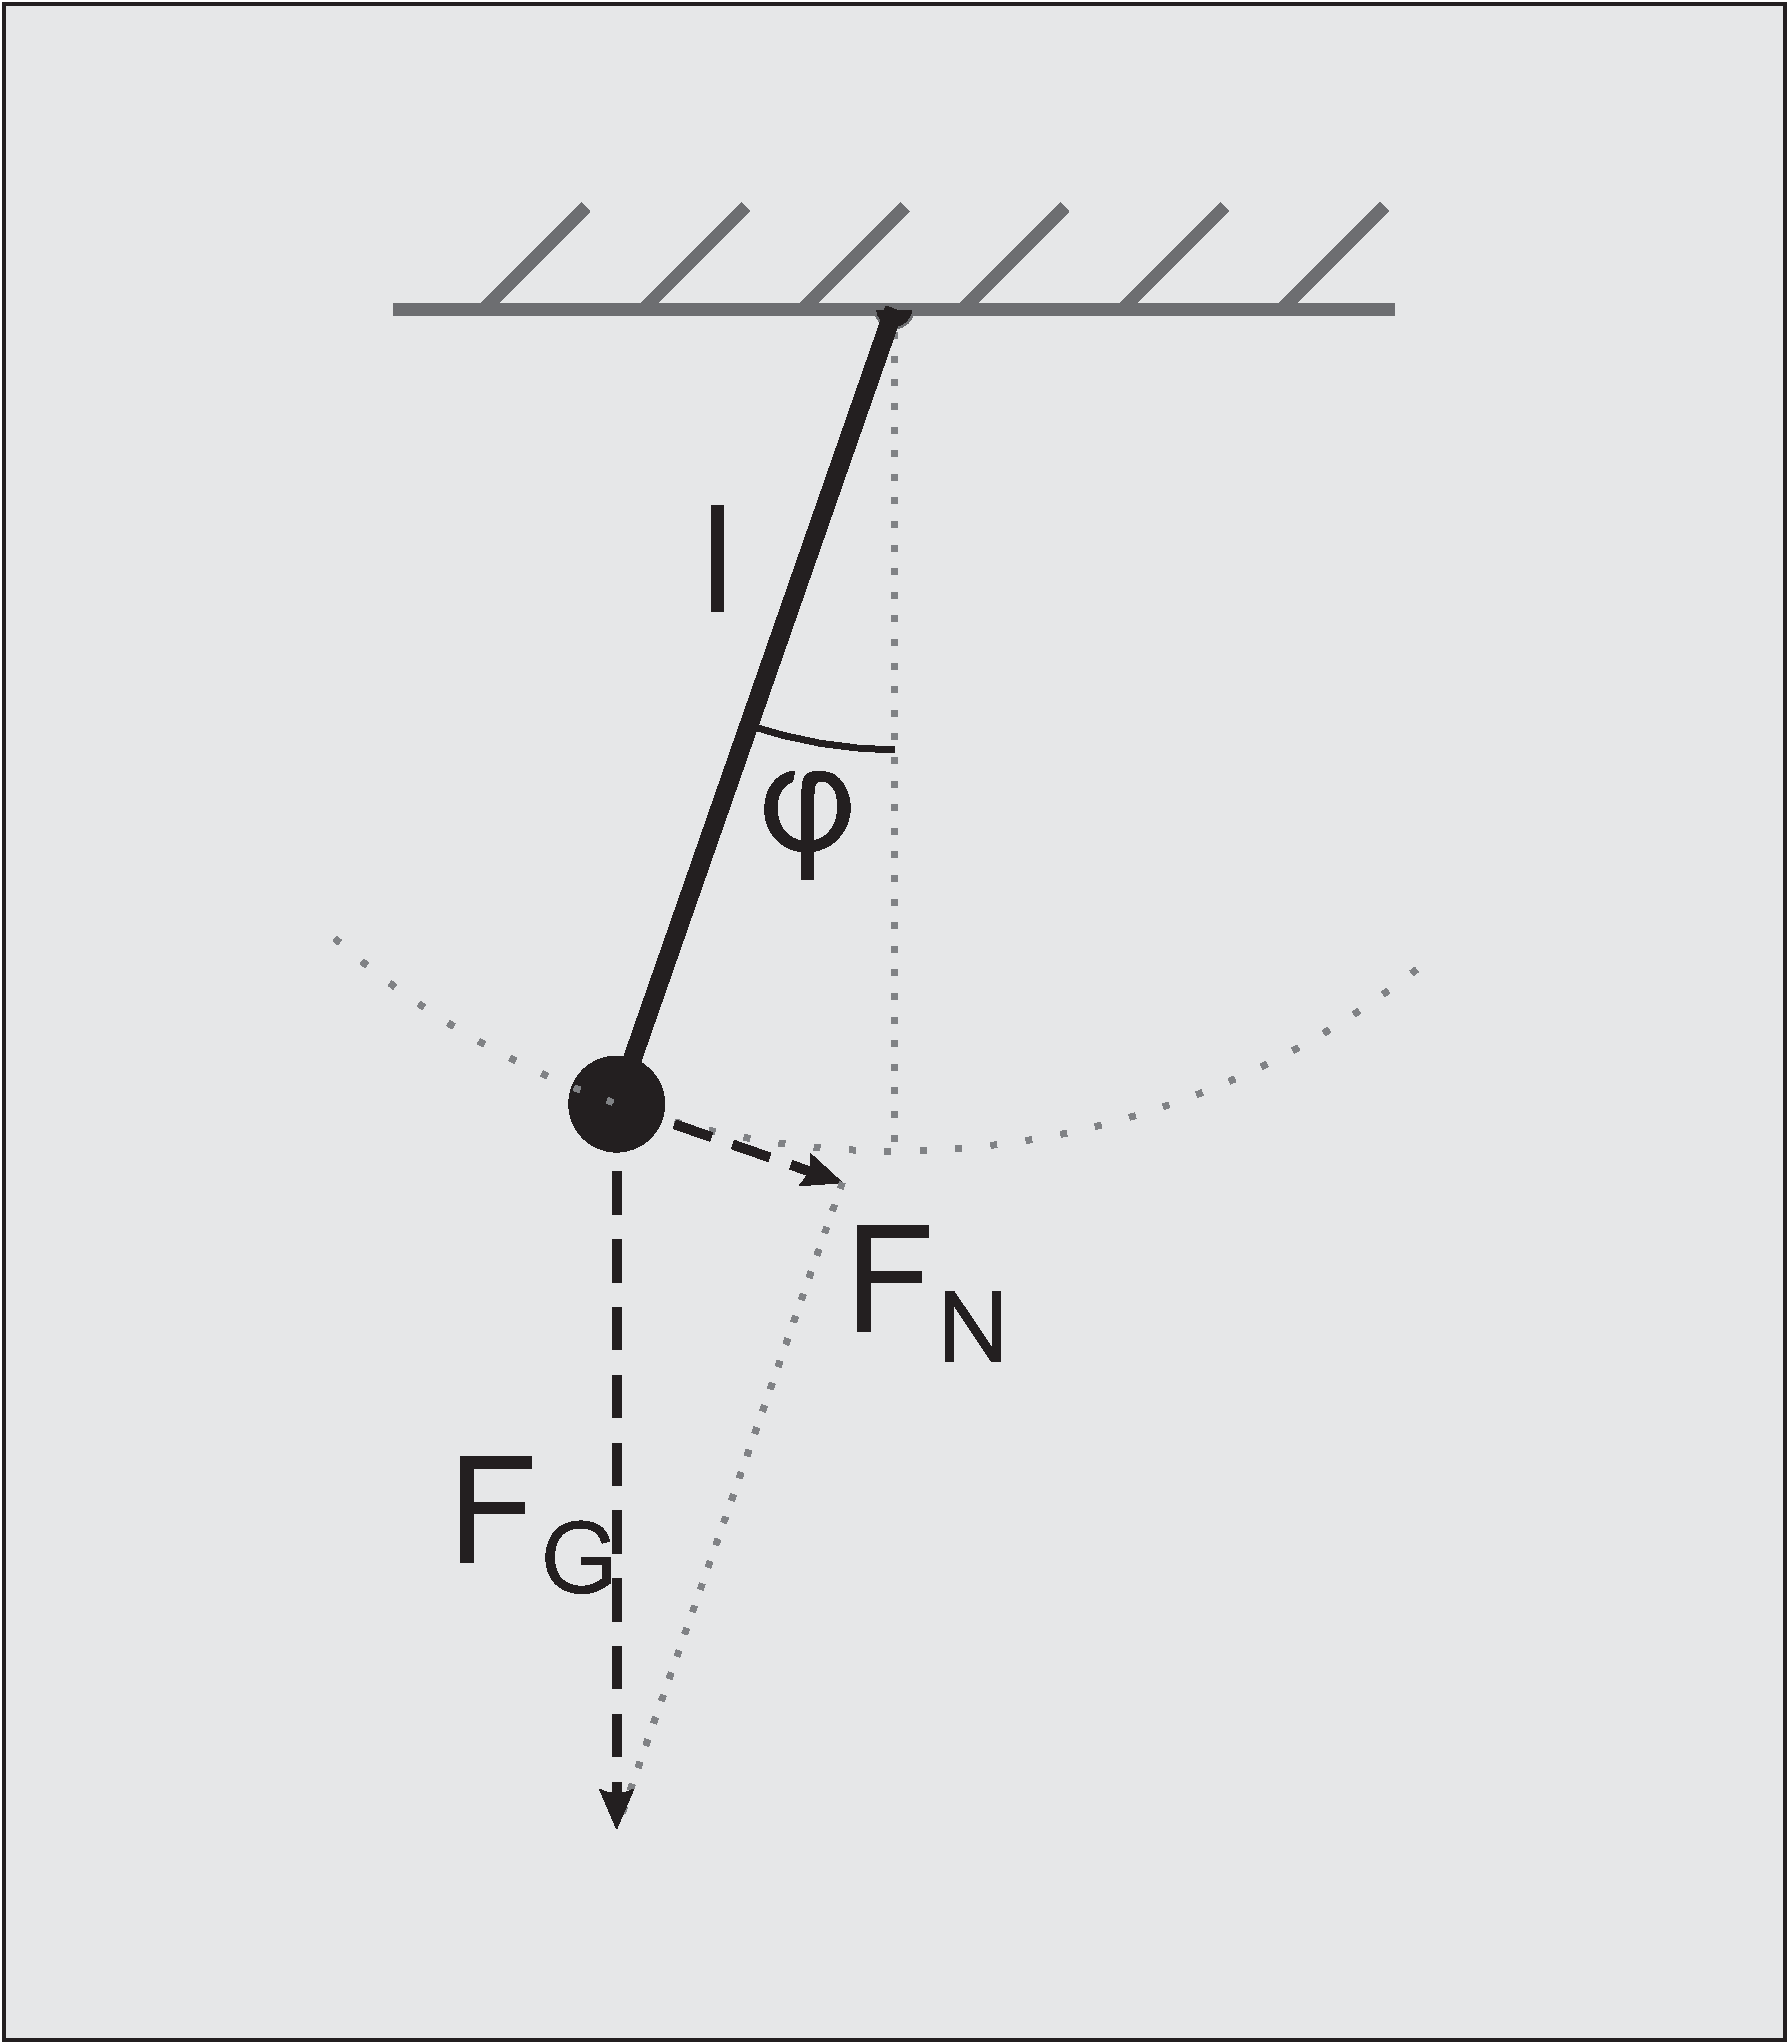
\includegraphics[draft=false,width=1.0\textwidth]{pendulum.pdf}
\end{minipage}
\hspace{2ex}
\begin{minipage}{0.5\textwidth}
 \only<1>{
 Pendulum -- Newtons law

 
 $m a = F$

 Acceleration

 $a = l \ddot{\varphi}$

 Force

 $F=F_N = - m g \sin \varphi$

 Result in an ode for the angle

 $\ddot{\varphi} = - g / l \sin \varphi $
 }

 \only<2>{

 $\ddot{\varphi} = - g / l \sin \varphi $

 Small angle $\sin \varphi \approx \phi$

 Harmonic oscillator

 $\ddot{\varphi} = - g / l \varphi$

 An analytic solution is known

 $\varphi = A \cos \omega t + B \sin \omega t$

 Amplitude $A$ and $B$ must be determined from initial conditions:

 $\varphi(t=0) = \varphi_0$, $\dot{\varphi}(t=0) = \dot{\varphi}_0$

 $B=\varphi_0$, $A=\dot{\varphi}_0 / \omega$

 }

 \only<3>{

 Full equation $\ddot{\varphi} = g / l \sin \varphi $

 has also analytic solution Jacobi elliptic function

 Lets enhance the ODE, add friction and external driving

 $\ddot{\varphi} = g / l \sin \varphi - \mu \dot{\varphi} + \varepsilon \sin \omega t $

 No analytic solution is known. We need to solve this equation numerically.

 }

 \only<4>{

 $\ddot{\varphi} = g / l \sin \varphi - \mu \dot{\varphi} + \varepsilon \sin \omega t $

 Create a first order ODE

 $x_1 = \varphi$, $x_2 = \dot{\varphi}$

 $\dot{x_1} = x_2$, $\dot{x_2} = - g / l \sin x_1 - \mu x_2 + \varepsilon \sin \omega t$

 $x_1$ and $x_2$ are the state space variables.

 }
 
\end{minipage}

 
\end{frame}


\begin{frame}[fragile]
 

\end{frame}
